\documentclass[xetex,mathserif,serif]{beamer}

% Language settings.
\usepackage{polyglossia}
\setdefaultlanguage[babelshorthands=true]{russian}

% Setting outer theme.
\useoutertheme{infolines}

% Setting font.
\usepackage{fontspec}
\setmainfont{FreeSans}
\newfontfamily{\russianfonttt}{FreeSans}

% Code highlighting.
\usepackage[outputdir=temp]{minted}
\usepackage{xcolor}

% Images.
\usepackage{graphicx}
\graphicspath{ {./images/} }

\title{Паттерн «Map-Reduce»}
\author[Александр Смирнов]{Александр Смирнов}
\date{10.03.2020}

\begin{document}

\begin{frame}
	\titlepage{}
\end{frame}

\begin{frame}[fragile]

	\frametitle{Введение}

	\begin{itemize}
		\item Техника для обработки больших данных
		\item map
		      \begin{itemize}
			      \item применяет функцию к каждому элементу последовательности и возвращает итератор с результатами
			      \item
			            \begin{minted}{python}
list(map(str.upper, ['one', 'two', 'list', '', 'dict']))
# ['ONE', 'TWO', 'LIST', '', 'DICT']

                        \end{minted}
			      \item
			            \begin{minted}{python}
list(map(lambda x: x + 1, [0, 2, 5]))
# [1, 3, 6]

                        \end{minted}
		      \end{itemize}
		\item reduce
		      \begin{itemize}
			      \item последовательно применяет функцию к элементам списка, возвращает единичное значение
			      \item
			            \begin{minted}{python}
reduce(lambda x, y: x + y, [1, 5, 9])
# 15

                        \end{minted}
			      \item
			            \begin{minted}{python}
reduce(lambda x, y: x if (x > y) else y, [1, 5, 9])
# 9

                        \end{minted}
		      \end{itemize}
	\end{itemize}
\end{frame}

\begin{frame}

	\frametitle{Пример}

	\begin{itemize}
		\item Вернуть самую длинную строку из списка строк
		\item На больших данных работает медленно
		\item Вертикальное масшабирование
		      \begin{itemize}
			      \item Внедрение более качественного и быстрого оборудования
			      \item Увеличение размера данных
		      \end{itemize}
		\item Горизонтальное масшабирование
		      \begin{itemize}
			      \item Разработаем код так, чтобы он мог работать параллельно
			      \item Станет быстрее, когда добавим процессоров
		      \end{itemize}
	\end{itemize}

\end{frame}

\begin{frame}

	\frametitle{Решение (1)}

	\begin{itemize}
		\item Разбить код на множество блоков
		\item Выполнить функцию поиска самой длинной строки для каждого блока параллельно
		\item Найти самую длинную строку среди выходных данных всех блоков
	\end{itemize}

\end{frame}

\begin{frame}

	\frametitle{Решение (2)}

	\begin{itemize}
		\item Разбили код на два этапа
		      \begin{itemize}
			      \item Вычисляем длину всех строк
			      \item Выбираем максимальное значение
		      \end{itemize}
		\item Дадим шагам имена
		      \begin{itemize}
			      \item mapper
			      \item reducer
		      \end{itemize}
		\item Разобъём входные данные на куски
		\item Распараллелим
	\end{itemize}

\end{frame}

\begin{frame}

	\frametitle{Архитектура}
	\begin{figure}[]
		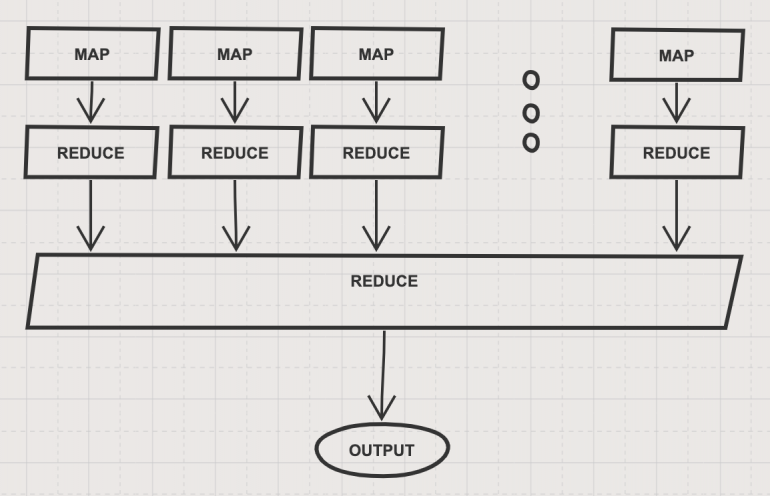
\includegraphics[scale=0.4]{architecture.png}
		\centering
	\end{figure}

	\begin{itemize}
		\item Каждый блок обрабатывает входные данные и reduce-ит их
		\item Результаты reduce-ов reduce-ятся
	\end{itemize}

\end{frame}

\begin{frame}

	\frametitle{Особенности}

	\begin{itemize}
		\item Масштабируемость
		      \begin{itemize}
			      \item Если больше данных, то просто добавляем больше процессоров без изменения кода
		      \end{itemize}
		\item Универсальность
		      \begin{itemize}
			      \item Поддерживается широкий спект задач, просто меняем функционал наших map и reduce
		      \end{itemize}
		\item Большие данные
		      \begin{itemize}
			      \item Разбиение на фрагметы неэффективно, поэтому будем хранить данные в виде кусков изначально
                  \item Hadoop Distributed File System
		      \end{itemize}
	\end{itemize}

\end{frame}
\end{document}
